\chapter{Sistema completo de fusión sensorial}
\label{cha:Sistema completo de fusión sensorial}

\begin{FraseCelebre}
  \begin{Frase}
    Texto.
  \end{Frase}
  \begin{Fuente}
    Autor texto
  \end{Fuente}
\end{FraseCelebre}

\section{Resumen de todo el modelo de detección 3D}
\label{sec:Resumen de todo el modelo de detección 3D}

Pasos eliminados respecto de  Frustum PointNets

Tiempos: Comparación con PointPainting (para mostrar hasta donde se puede mejorar el tiempo de las transformaciones geométricas)

\begin{table}[H]
\centering
\begin{tabular}{|lr|}
\hline
YOLOv5                       & 10.79 ms                     \\ \hline
Aproximación de la distancia & 10.65 ms                     \\ \hline
Generación del frustum       & 9.09 ms                      \\ \hline
FrustumPP                    & 10.87 ms                     \\ \hline
Transformación final         & 0.45 ms                      \\ \hline \hline
\textbf{TOTAL}               & \textbf{41.85 ms (23.89 Hz)} \\ \hline
\end{tabular}
\end{table}

1245 MBs de memoria de vídeo necesaria

\section{Resultados obtenidos en KITTI}
\label{sec:Resultados obtenidos en KITTI}

\begin{figure}[H]
	\begin{minipage}{0.333\textwidth}
		\centering
		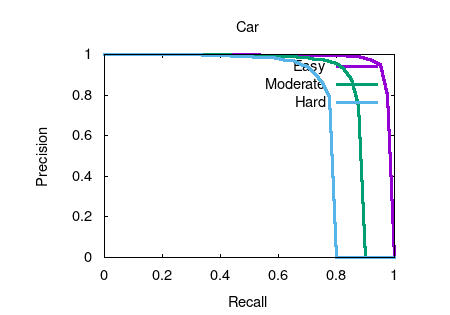
\includegraphics[width=1\linewidth]{Book/figures/9_completo/car_detection_ground.png}
	\end{minipage}\hfill
	\begin{minipage}{0.333\textwidth}
		\centering
		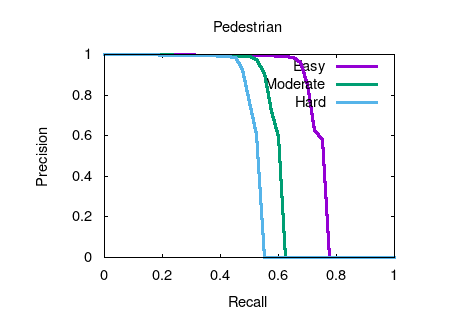
\includegraphics[width=1\linewidth]{Book/figures/9_completo/pedestrian_detection_ground.png}
	\end{minipage}\hfill
	\begin{minipage}{0.333\textwidth}
		\centering
		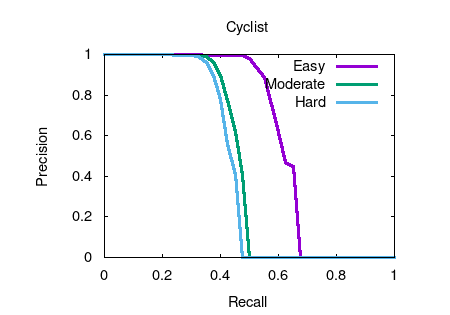
\includegraphics[width=1\linewidth]{Book/figures/9_completo/cyclist_detection_ground.png}
	\end{minipage}
	\caption{Curvas PR del modelo completo sobre la tarea de detección en BEV.}
	\label{fig:Curvas PR del modelo completo sobre la tarea de detección en BEV.}
\end{figure}

\begin{figure}[H]
	\begin{minipage}{0.333\textwidth}
		\centering
		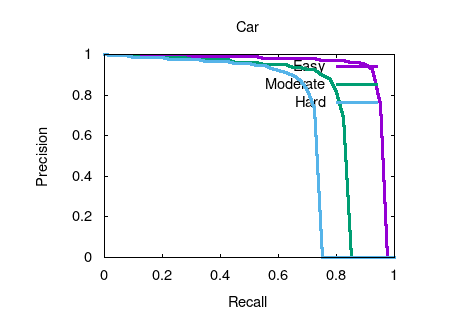
\includegraphics[width=1\linewidth]{Book/figures/9_completo/car_detection_3d.png}
	\end{minipage}\hfill
	\begin{minipage}{0.333\textwidth}
		\centering
		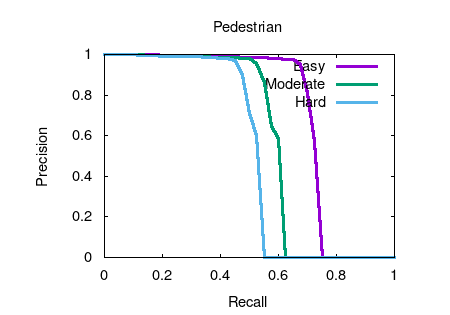
\includegraphics[width=1\linewidth]{Book/figures/9_completo/pedestrian_detection_3d.png}
	\end{minipage}\hfill
	\begin{minipage}{0.333\textwidth}
		\centering
		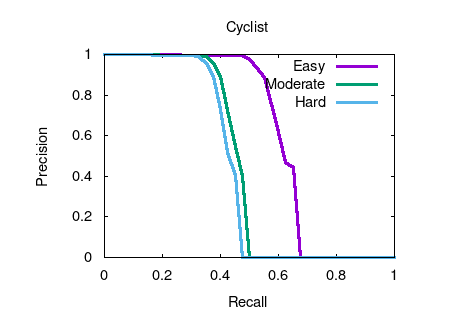
\includegraphics[width=1\linewidth]{Book/figures/9_completo/cyclist_detection_3d.png}
	\end{minipage}
	\caption{Curvas PR del modelo completo sobre la tarea de detección 3D.}
	\label{fig:Curvas PR del modelo completo sobre la tarea de detección 3D.}
\end{figure}

\begin{figure}[H]
  \begin{subfigure}[t]{.48\textwidth}
    \centering
    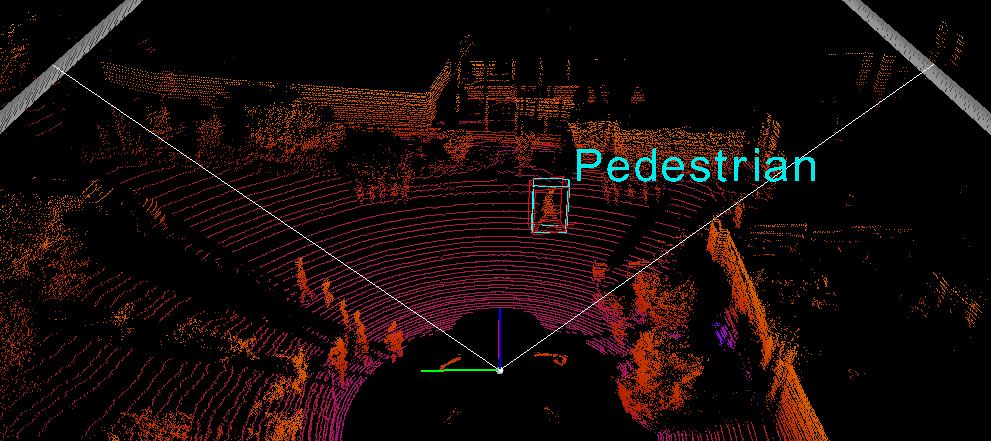
\includegraphics[width=\linewidth]{Book/figures/9_completo/complete_0.png}
  \end{subfigure}
  \hfill
  \begin{subfigure}[t]{.48\textwidth}
    \centering
    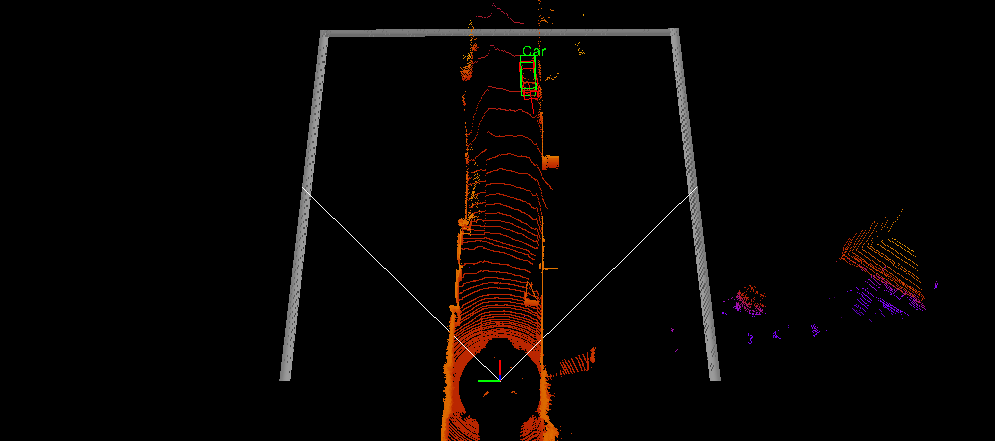
\includegraphics[width=\linewidth]{Book/figures/9_completo/complete_1.png}
  \end{subfigure}
  \bigbreak
  \begin{subfigure}[t]{.48\textwidth}
    \centering
    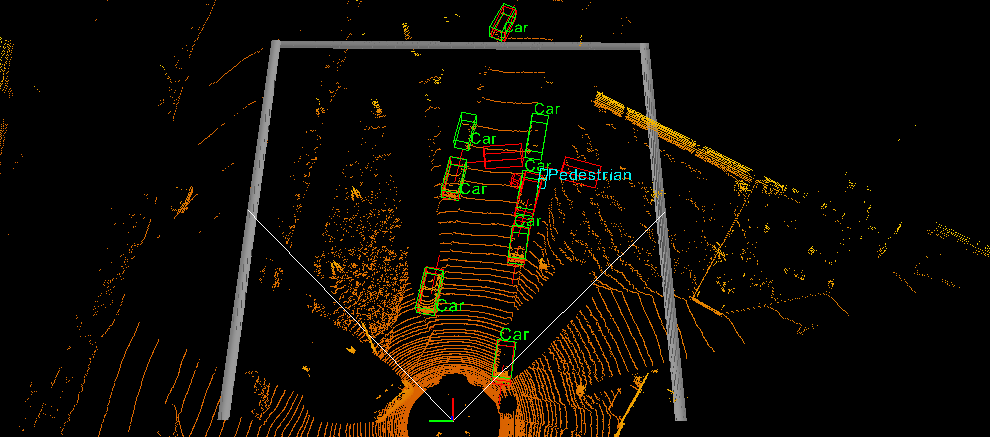
\includegraphics[width=\linewidth]{Book/figures/9_completo/complete_2.png}
  \end{subfigure}
  \hfill
  \begin{subfigure}[t]{.48\textwidth}
    \centering
    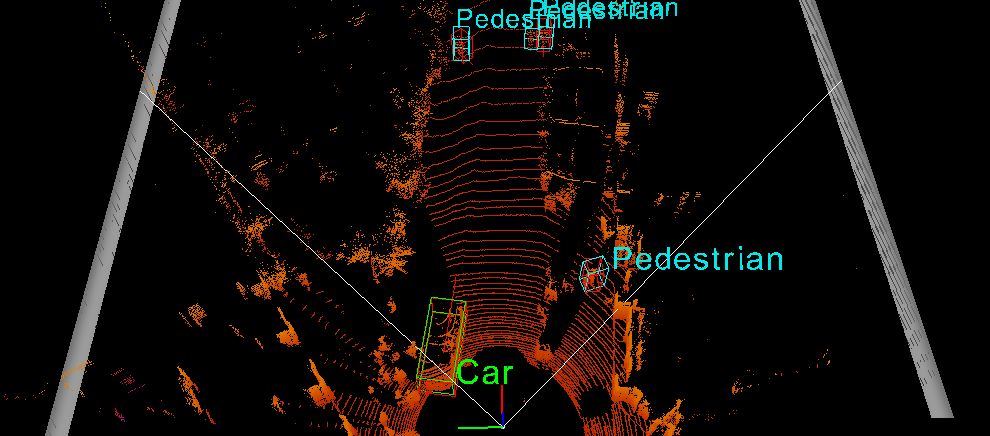
\includegraphics[width=\linewidth]{Book/figures/9_completo/complete_3.png}
  \end{subfigure}
\caption{Detecciones 3D obtenidas sobre las nubes de puntos de KITTI.}
\label{fig:Detecciones 3D obtenidas sobre las nubes de puntos de KITTI.}
\end{figure}

\begin{figure}[H]
  \begin{subfigure}[t]{.48\textwidth}
    \centering
    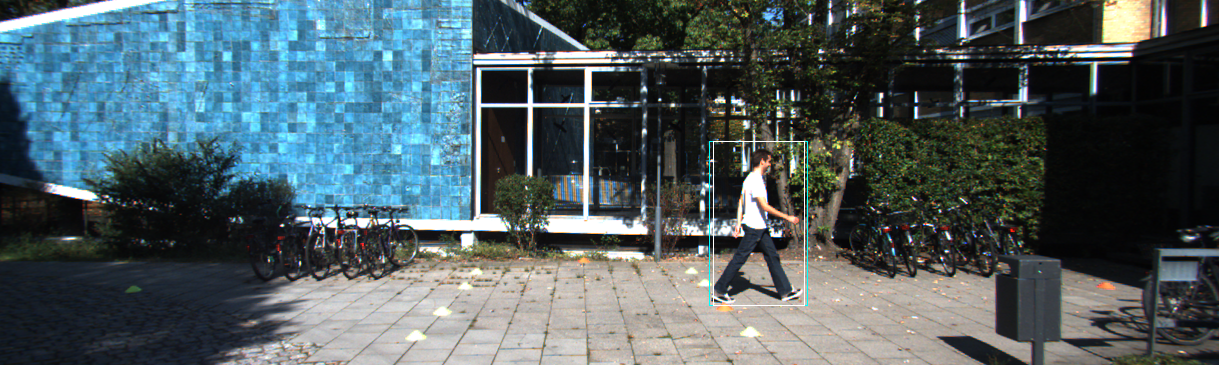
\includegraphics[width=\linewidth]{Book/figures/9_completo/kitti_image_0.png}
  \end{subfigure}
  \hfill
  \begin{subfigure}[t]{.48\textwidth}
    \centering
    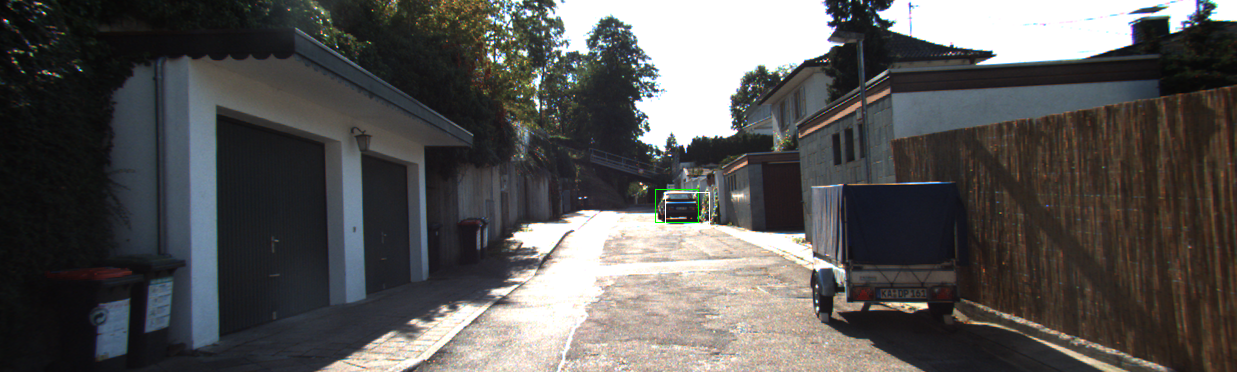
\includegraphics[width=\linewidth]{Book/figures/9_completo/kitti_image_1.png}
  \end{subfigure}
  \bigbreak
  \begin{subfigure}[t]{.48\textwidth}
    \centering
    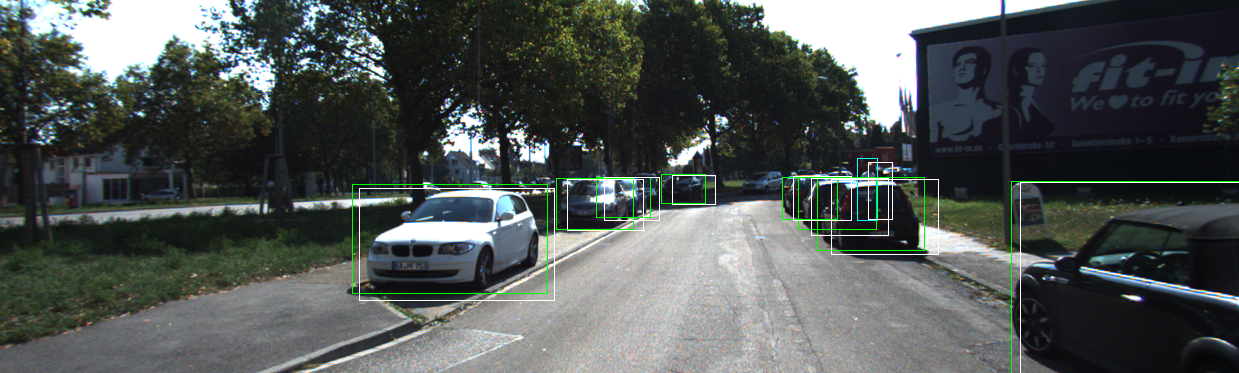
\includegraphics[width=\linewidth]{Book/figures/9_completo/kitti_image_2.png}
  \end{subfigure}
  \hfill
  \begin{subfigure}[t]{.48\textwidth}
    \centering
    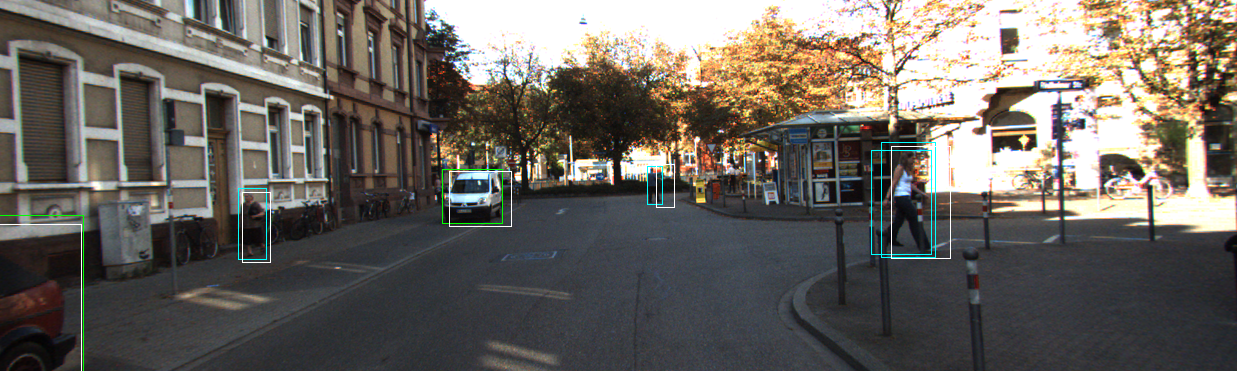
\includegraphics[width=\linewidth]{Book/figures/9_completo/kitti_image_3.png}
  \end{subfigure}
\caption{Detecciones 2D utilizadas para la obtención de las detecciones 3D.}
\label{fig:Detecciones 2D utilizadas para la obtención de las detecciones 3D.}
\end{figure}